\chapter{Modelling proton-proton interactions}
\label{ch:MC}

For any measurement in particle physics, sets of simulated samples need to be generated in order to compare the experimental data to theoretical models.  
These models include well known \SM{} decay processes such as \ttbar{} production, much rarer processes predicted by the \SM{} such as $\mathrm{t}\overline{\mathrm{t}}\mathrm{H}}$ and in the case of a search for new physics a plethora of processes predicted by \BSM{} theories.

These different processes are modelled by event generators in a similar manner, following a sequence of discrete steps.
First of all, a possible hard scattering interaction is generated for a process at \LO{}, or if possible \NLO{}.
If short-lived resonances are formed, their associated decays are also viewed as part of the hard process.
Additional parton interactions can be included at \LO{} and soft radiation added to the initial and final states, in a process known as the \textit{parton shower}.
The parton shower is then hadronised into colourless states and decayed, with the proton remnants forming the underlying event.
Figure~\ref{fig:GenEvent} shows diagrammatically an example simulated collision, where the hard scattering process is shown in red, the soft radiative processes in blue, the additional parton interactions in purple, the fragmentation in light green and hadronisation and decay in dark green.
Photon radiation is shown in yellow.
Finally, the interactions of the particles produced with the detector can be modelled and the detector response applied.
\begin{figure}[htpb]
	\centering
	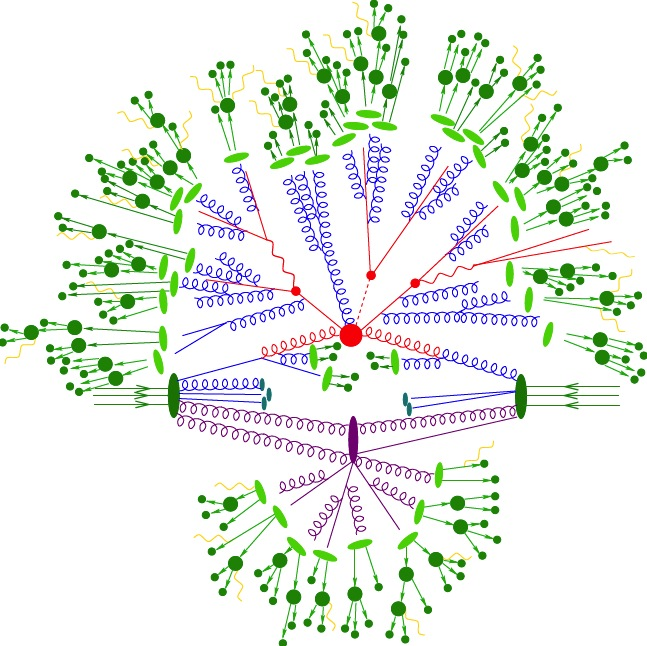
\includegraphics[width=\textwidth]{Figures/Generator_Event}
	\caption[An example simulation of a proton-proton collision showing all the various processes that must be modelled. Starting with the hard interaction in red calculated using perturbation theory, then dressing with additional soft processes in blue forming the parton shower. Additional parton interactions are added, shown in purple, each with a respective parton shower. Finally the parton shower is fragmented and hadronised into detectable, colourless hadrons, which can in turn decay and radiate. This fragmentation and hadronisation processes are shown in light green and green respectively. Photon radiation is shown in yellow. ]{An example simulation of a proton-proton collision showing all the various processes that must be modelled. Starting with the hard interaction in red calculated using perturbation theory, then dressing with additional soft processes in blue forming the parton shower. Additional parton interactions are added, shown in purple, each with a respective parton shower. Finally the parton shower is fragmented and hadronised into detectable, colourless hadrons, which can in turn decay and radiate. This fragmentation and hadronisation processes are shown in light green and green respectively. Photon radiation is shown in yellow.  Figure taken from~\cite{Gen:Event}.}
	\label{fig:GenEvent}
\end{figure}

\section{Hard interaction} % (fold)
\label{sec:hard_interaction}
The hard scattering process describes the interaction of two partons in the collider.
It is modelled through Eq~\ref{eq:pdf}, with the \PDF{}s taken from data convoluted with the partonic cross section.
The partonic cross section is calculated from the matrix-element of the interaction, directly taken from the Feynman diagrams through the Feynman rules.
If a short-lived resonance is formed as a result of the interaction, then its decay is also considered as part of the hard interaction.
Many matrix-elements can already be calculated to \NNLO{} or higher, however the generation of the hard scattering processes can currently only be calculated to \LO{} or \NLO{}.
This is simply due to the combinatorics when taking into account all possible Feynman diagrams.

There are a variety of matrix-element generators available, two of the most popular in high energy particle physics being MadGraph5\_aMC@NLO (\mgamc{})~\cite{Gen:MGamc} and POsitive Weight Hardest Emission Generator (\powheg{})~\cite{Gen:Pow1,Gen:Pow2,Gen:Pow3}.
The \mgamc{} matrix-element generator can model a process with additional partons.
The number of additional partons in the process depends on the complexity of the process, \eg{} for \NLO{} \ttbar{} production, an additional two partons can be generated.
It does this by adding real diagrams based on \LO{} or \NLO{} contributions from lower order processes.
In \powheg{}, virtual processes are included in the matrix element, up to one loop. 
This means that for \ttbar{} production, one less additional parton is able to be produced.
% Madgraph. Depending on the process a number of additional partons can be generated.
% at NLO
% e.g. tt at NLO: real contributions with respect to LO
% e.g. ttj at NLO: real NLO diagrams wrt tt at NLO
% e.g. ttjj at NLO: real NNLO diagrams wrt tt at NLO and real NLO diagrams wrt ttj at NLO
% at LO
% e.g. tt at LO: tree diagram
% e.g. ttj at LO: real NLO diagrams wrt tt at LO
% e.g. ttjj at LO: real NNLO diagrams wrt tt at LO and real NLO diagrams wrt ttj at LO
% e.g. ttjjj at LO: real NNNLO diagrams wrt ttjj at LO and real NNLO diagrams wrt ttj at LO and real NLO diagrams wrt ttj at LO


% section hard_interaction (end)

\section{Additional interactions and soft processes} % (fold)
\label{sec:additional_interactions_and_soft_processes}

Once the hard process has been simulated from the matrix-element calculations, additional hard, low-\pt{}, interactions need to be included. 
All the hard interactions then present in the simulation must be \textit{dressed} with soft emissions.

The most common hard process at the LHC is elastic gluon-gluon scattering, the cross section of which, diverges as the gluons become soft and collinear.
This means that below some momentum transfer threshold ($\sim5\GeV$) the inclusive jet production cross section from elastic gluon-gluon scattering is larger than the total inclusive proton-proton cross section~\cite{Gen:MPI_1, Gen:MPI_2}, which infers that for every collision, more than one interaction is occurring.
These are known as \textit{multiple parton interactions} (\MPI{}).
The number of additional interactions present is proportional to the impact parameter of the colliding protons.
A pair of protons colliding head on contains more additional interactions than a pair that collide obliquely.
% elastic = total here. dominated by t-channel processes

The extra soft emissions come in the form of \textit{initial} and \textit{final state radiation} (\ISR{} and \FSR{}), where partons split from the hard interactions.
Figure~\ref{fig:feyn-ps} shows the four possible ways in which a parton can be radiated.
Firstly, a quark can radiate a gluon, secondly a gluon can pair-produce a \qqbar{} pair and finally there are two colour configurations of gluon splitting.
\begin{figure}[h!]
	\centering
	\begin{resizedtikzpicture}{0.45\linewidth}
		\begin{feynman}
			\vertex (A);
			\vertex [above=0.015cm of A] (aup);
			\vertex [below=0.015cm of A] (adown);

			\vertex [right=1.5cm of A] (B);
			\vertex [above=0.015cm of B] (bup);
			\vertex [below=0.015cm of B] (bdown);

			\vertex [above right=0.75cm and 1.5cm of B] (C);
			\vertex [above=0.015cm of C] (cup);
			\vertex [below=0.015cm of C] (cdown);
			\vertex [below right=0.75cm and 1.5cm of B] (D);
			\vertex [above=0.015cm of D] (dup);
			\vertex [below=0.015cm of D] (ddown);

			\diagram*{
			% (bup) -- [red,thick,edge label=\(\overline{r}\)] (dup),
			% (ddown) -- [electricgreen,thick,edge label=\(g\)] (bdown),
			% (B) -- [red,very thick,edge label=\(r\)] (C),
			% (A) -- [electricgreen,very thick,edge label=\(g\)] (B),
			(bup) -- [red,thick] (dup),
			(ddown) -- [electricgreen,thick] (bdown),
			(B) -- [red,very thick] (C),
			(A) -- [electricgreen,very thick] (B),
			(A) -- [fermion] (B),
			(B) -- [fermion] (C),
			(B) -- [gluon] (D),
			};
		\end{feynman}
		\end{resizedtikzpicture}
		\hspace{0.5cm}
		\begin{resizedtikzpicture}{0.45\linewidth}
		\begin{feynman}
			\vertex (A);
			\vertex [above=0.015cm of A] (aup);
			\vertex [below=0.015cm of A] (adown);

			\vertex [right=1.5cm of A] (B);
			\vertex [above=0.015cm of B] (bup);
			\vertex [below=0.015cm of B] (bdown);

			\vertex [above right=0.75cm and 1.5cm of B] (C);
			\vertex [above=0.015cm of C] (cup);
			\vertex [below=0.015cm of C] (cdown);
			\vertex [below right=0.75cm and 1.5cm of B] (D);
			\vertex [above=0.015cm of D] (dup);
			\vertex [below=0.015cm of D] (ddown);

			\diagram*{
			(aup) -- [red,thick] (bup),
			(adown) -- [electricgreen,thick] (bdown),
			(B) -- [red,very thick] (C),
			(B) -- [electricgreen,very thick] (D),

			(A) -- [gluon] (B),
			(B) -- [fermion] (C),
			(B) -- [anti fermion] (D),
			};
		\end{feynman}
		\end{resizedtikzpicture} \\
		\vspace{0.5cm}
		\begin{resizedtikzpicture}{0.45\linewidth}
		\begin{feynman}
			\vertex (A);
			\vertex [above=0.015cm of A] (aup);
			\vertex [below=0.015cm of A] (adown);

			\vertex [right=1.5cm of A] (B);
			\vertex [above=0.015cm of B] (bup);
			\vertex [below=0.015cm of B] (bdown);
			\vertex [right=0.025cm of B] (bright);
			\vertex [above=0.015cm of bright] (brightup);
			\vertex [below=0.015cm of bright] (brightdown);

			\vertex [above right=0.75cm and 1.5cm of B] (C);
			\vertex [above=0.015cm of C] (cup);
			\vertex [below=0.015cm of C] (cdown);
			\vertex [below right=0.75cm and 1.5cm of B] (D);
			\vertex [above=0.015cm of D] (dup);
			\vertex [below=0.015cm of D] (ddown);

			\diagram*{
			(bup) -- [red,thick] (cup),
			(bdown) -- [electricgreen,thick] (ddown),
			(bright) -- [blue,thick,sharp arrow angle=60,sharp right-] (cdown),
			(bright) -- [blue,thick,sharp arrow angle=60,sharp left-] (dup)
			(aup) -- [red,thick,sharp arrow angle=45,-sharp right] (brightup),
			(adown) -- [electricgreen,thick,sharp arrow angle=45,-sharp left] (brightdown),
			(A) -- [gluon] (B),
			(B) -- [gluon] (C),
			(B) -- [gluon] (D),
			};
		\end{feynman}
		\end{resizedtikzpicture}
		\hspace{0.5cm}
		\begin{resizedtikzpicture}{0.45\linewidth}
		\begin{feynman}
			\vertex (A);
			\vertex [above=0.015cm of A] (aup);
			\vertex [below=0.015cm of A] (adown);

			\vertex [right=1.5cm of A] (B);
			\vertex [above=0.015cm of B] (bup);
			\vertex [below=0.015cm of B] (bdown);
			\vertex [right=0.025cm of B] (bright);
			\vertex [above=0.015cm of bright] (brightup);
			\vertex [below=0.015cm of bright] (brightdown);

			\vertex [above right=0.75cm and 1.5cm of B] (C);
			\vertex [above=0.015cm of C] (cup);
			\vertex [below=0.015cm of C] (cdown);
			\vertex [below right=0.75cm and 1.5cm of B] (D);
			\vertex [above=0.015cm of D] (dup);
			\vertex [below=0.015cm of D] (ddown);

			\diagram*{
			(bright) -- [red,thick,sharp arrow angle=60,sharp left-] (dup),
			(bright) -- [electricgreen,thick,sharp arrow angle=60,sharp right-] (cdown),
			(bup) -- [blue,thick] (cup),
			(bdown) -- [blue,thick] (ddown),
			(aup) -- [red,thick,sharp arrow angle=45,-sharp right] (brightup),
			(adown) -- [electricgreen,thick,sharp arrow angle=45,-sharp left] (brightdown),
			(A) -- [gluon] (B),
			(B) -- [gluon] (C),
			(B) -- [gluon] (D),
			};
		\end{feynman}
		\end{resizedtikzpicture}
	\caption[The four possible processes to strongly split a parton in the parton shower. The top left panel shows gluon emission, the top right shows \qqbar{} pair production and the bottom two panels the colour configurations of gluon splitting. In addition, photon brehmsstrahlung from the quarks can occur but is not considered here.]{The four possible processes to strongly split a parton in the parton shower. The top left panel shows gluon emission, the top right shows \qqbar{} pair production and the bottom two panels the colour configurations of gluon splitting. In addition, photon brehmsstrahlung from the quarks can occur but is not considered here. }
	\label{fig:feyn-ps}
\end{figure}

For \FSR{}, the partons produced from the matrix-element calculation are split recursively until the energy of each remaining parton reduces to approximately 1\GeV{}, whereupon hadronisation effects become non-negligible.
In contrast, the \ISR{} is modelled differently.
The longitudinal momentum fractions, $x_1$ and $x_2$, of the incoming partons are taken from the \PDF{} at the factorisation scale of the process and evolved backwards in time. 
The factorisation scale of an event is a cutoff where partons that carry a momentum less than the cutoff scale are absorbed into the \PDF{}.
If the momentum carried is above the scale then they participate in the interaction.
This ensures no divergences in the matrix-element due to collinear or soft gluons.
For every \ISR{} emission, the parent parton must have the combined energy of the daughter parton and radiation.
There are however, fewer available partons carrying the increased fraction of the proton momentum, seen in the \PDF{} distribution, and so a suppression weight must be applied.
The suppression weight is derived from the \textit{Sudakov form factors}~\cite{Gen:Sudokov}.
In practice, the application of \ISR{} and \MPI{} occur completely and in tandem, before the \FSR{} is modelled.

The collective spray of partons produced by the hard process, \MPI{}, \ISR{} and \FSR{} is called the parton shower.
The evolution of the splittings in the parton shower is defined by ordering variables.
One such shower ordering variable is the square of the \pt{} of the shower propagators (\ktsq{}), such that \ktsq{} for a daughter splitting is less than the \ktsq{} for a mother splitting~\cite{Gen:kt}.
The splittings between \MPI{} can also be interleaved with one another.
The \ktsq{} ordering is illustrated in the left panel of Fig.~\ref{fig:feyn-ordering}, where the hard interaction occurs at $Q_{max}$ and the splitting strengths, given by $V_{i}(\ktsq{})$, are ordered $V_{1} > V_{2} > V_{3}$ (The further in time from the hard interaction, the softer and more collinear the splitting). 

Another way to evolve the shower is by using an angular ordering~\cite{Gen:angular}.
This angular ordering requires any future splitting to occur within a cone defined by the angular radius between the daughter partons from the previous splitting also illustrated in the right panel of Fig.~\ref{fig:feyn-ordering}.
These showers often produce wide-angle soft splittings before the main hard splitting.
% as would be the case in a \ktsq{}-ordered shower.
Two widely used models for the parton shower are \pythia{}~\cite{Gen:Pyth8p2} and \herwig{}~\cite{Gen:Herwigpp}, where \pythia{} uses a \ktsq{}-ordered shower and \herwig{} an angular-ordered shower.
\begin{figure}[h!]
\centering
\begin{resizedtikzpicture}{0.4\linewidth}
	\begin{feynman}
		\vertex (A);
		\vertex [right=1cm of A](C);
		\vertex [above=1.5cm of C](Ci);
		\vertex [below=0.05cm of C](C_quiet){\(V_{2}\)};
		\vertex [right=2.0cm of C](D);
		\vertex [above=0.05cm of D](D_quiet){\(Q_{max}\)};
		\vertex [right=2.5cm of D](F);
		\vertex [below=1.5cm of F](Fi);
		\vertex [left=0.05cm of Fi](F_quiet){\(V_{3}\)};
		\vertex [above right=0.75 cm and 1.5cm of Fi](Fii);
		\vertex [below right=0.75 cm and 1.5cm of Fi](Fiii);
		\vertex [right=1.5cm of F](G);

		\vertex [below=3cm of A](B);
		\vertex [right=3cm of B](E);
		\vertex [below=0.05cm of E](E_quiet){\(Q_{max}\)};
		\vertex [right=1.5cm of E](H);
		\vertex [above=0.05cm of H](H_quiet){\(V_{1}\)};
		\vertex [below=1.5cm of H](Hi);
		\vertex [right=2.5cm of H](I);

		\diagram* {
		(A) -- [fermion] (C),
		(C) -- [gluon] (Ci),
		(C) -- [fermion] (D),
		(D) -- [fermion] (F),
		(F) -- [gluon] (Fi),
		(Fi) -- [fermion] (Fii),
		(Fi) -- [anti fermion] (Fiii),
		(F) -- [fermion] (G),

		(B) -- [fermion] (E),
		(E) -- [fermion] (H),
		(H) -- [gluon] (Hi),
		(H) -- [fermion] (I),

		(D) -- [gluon] (E),
		};
	\end{feynman}
\end{resizedtikzpicture}
\hspace{0.4cm}
\begin{resizedtikzpicture}{0.56\linewidth}
	\begin{feynman}
		\vertex (A);
		\vertex [right=0.5cm of A](A_quiet){\(\theta_{max}\)};
		\vertex [left=1.5cm of A](Aminus);
		\vertex [below right=1.5cm and 1.5cm of A](A2);
		\vertex [above right=1.5cm and 1.5cm of A](B);
		\vertex [above right=0.2cm and 0.2cm of B](B_quiet){\(\theta_{1}\)};
		\vertex [above=1.5cm of B](C);
		\vertex [right=2.25cm of B](D);
		\vertex [right=0.5cm of D](D_quiet){\(\theta_{2}\)};
		\vertex [above right=1.25cm and 2.25cm of D](E);
		\vertex [above right=0.5cm and 1.25cm of E](E_quiet){\(\theta_{3}\)};
		\vertex [below right=1.25cm and 2.25cm of D](F);
		\vertex [below right=0.5cm and 1.25cm of F](F_quiet){\(\theta_{4}\)};
		\vertex [above right=1.5cm and 1.75cm of E](G);
		\vertex [above right=0.5cm and 2.25cm of E](H);
		\vertex [below right=1.5cm and 1.75cm of F](I);
		\vertex [below right=0.5cm and 2.25cm of F](J);

		\diagram* {
		(Aminus) -- [gluon] (A),
		(A) -- [anti fermion] (A2),
		(A) -- [fermion] (B),
		(B) -- [gluon] (C),
		(B) -- [fermion] (D),
		(D) -- [gluon] (E),
		(D) -- [fermion] (F),
		(E) -- [fermion] (G),
		(E) -- [anti fermion] (H),
		(F) -- [fermion] (I),
		(F) -- [gluon] (J),
		};
	\end{feynman}
\end{resizedtikzpicture}
\caption[The left panel shows parton shower ordering by \ktsq{} where the splitting strength $V_{i}(\ktsq)$ is ordered $V_1 > V_2 > V_3$. The right panel shows shower ordering by angle such that the opening angle decreases for every consecutive splitting $\theta_{max} > \theta_{1} > \theta_{2} > \theta_{3, 4}$.]{The left panel shows parton shower ordering by \ktsq{} where the splitting strength $V_{i}(\ktsq)$ is ordered $V_1 > V_2 > V_3$. The right panel shows shower ordering by angle such that the opening angle decreases for every consecutive splitting $\theta_{max} > \theta_{1} > \theta_{2} > \theta_{3, 4}$.}
\label{fig:feyn-ordering}
\end{figure}


% http://citeseerx.ist.psu.edu/viewdoc/download?doi=10.1.1.575.1213&rep=rep1&type=pdf
% http://www.hep.phy.cam.ac.uk/seminars/talks/2008/michaelmas/PaoloNason-14102008.pdf
% https://indico.cern.ch/event/35476/contributions/1760582/attachments/703609/965976/krauss_showers.pdf
% http://cds.cern.ch/record/694095/files/0312274.pdf
% http://www.iaea.org/inis/collection/NCLCollectionStore/_Public/45/031/45031526.pdf
% https://arxiv.org/pdf/1411.4085.pdf
% section additional_interactions_and_soft_processes (end)


\section{Matching matrix-elements to parton showers} % (fold)
\label{sec:matching_matrix_elements_to_parton_showers}

Parton showers and higher-order matrix-element calculations describe the same physics and so need to be combined consistently.
The soft emissions added from the parton shower should interface with the matrix-element based radiation with no gaps or overlaps for a specific, fixed final state parton multiplicity.
This problem is solved by a process known as \textit{matching}.
% TODO MERGING?

One method of matching, known as the \MLM{}-method~\cite{Gen:MLM}, after its author M. L. Mangano, matches the final state partons produced by the matrix-element calculation to parton jets created by clustering the showered partons.
The angular distance from each final state parton to each parton jet, starting from the parton with the leading \pt{}, is calculated and is said to be matched if it is less than a threshold value.
If the matching is successful the parton jet is removed from further calculations.
All final state partons must be matched to parton jets, otherwise the event is rejected.
When simulating the hard interaction process, including contributions with up to $N$ additional partons, events in samples simulated with $n$ additional partons, where $n<N$, are suppressed if they do not contain exactly $n$ matched parton jets.
This is because these events are present and more accurately modelled in the $n+1$ production sample and thus double counting is avoided.
All the production samples generated using discrete additional parton multiplicities are subsequently \textit{merged}.

When matching and merging at \NLO{} the additional parton jet from the matrix-element calculation is the hardest emission and thus defines the upper shower scale level.
While it is easy to interface this with showers ordered to some \pt{}, care must be taken with respect to an angular-ordered shower.
Angular-ordered shower emissions with a \pt{} greater than the additional matrix-element parton jet need to be suppressed.
The \FxFx{}-method~\cite{Gen:FXFX}, extends the \MLM{}-method of merging to matrix-elements calculated to \NLO{}.
The \MLM{}-method is used when matching \LO{} \mgamc{} to \pythia{} and the \FxFx{}-method is used when matching \NLO{} \mgamc{} to \pythia{}.

When \powheg{} models processes at a large factorisation scale, the number of high-\pt{} soft emissions is overestimated. 
It is resolved by introducing a \pt{} dependent damping factor, 
\begin{equation*}
	D = \frac{\hdamp^2}{\pt^2+\hdamp^2},
\end{equation*}
where \hdamp{} is the damping parameter, usually set to the factorisation scale (in the case for top quark production to $m_t$).
$D$ effectively sets the upper-\pt{} limit for the first additional emission and hence the upper shower scale level.

% Either start with higher Q2 in parton and evolve forwards. 
% Inefficient as prob here of this is small. 
% Or start with lower Q2 and evolve backwards.
% Matching - procedure to obtain a smooth transition for a fixed parton multiplicity
% Merging - the combination of several multiplicities
% Discarded e.g. if two partons match to the same jet (merged) or if parton not energetic enough to produce a jet.

% section matching_matrix_elements_to_parton_showers (end)

\section{Fragmentation and colour reconnection} % (fold)
\label{sec:fragmentation_and_colour_reconnection}

The fragmentation process models how final state partons from the parton shower hadronise into colourless states.
There are two general methods in use for the fragmentation, the \textit{Lund string model}~\cite{Gen:LundString1,Gen:Pyth8p2} and the \textit{cluster model}~\cite{Gen:Herwigpp}.

\subsection{Lund string model} % (fold)
\label{sub:string_fragmentation}

Due to the self interactions of gluons, the strong field between two quarks can be represented by a confined tube of dimension $1+1$, otherwise known as a string. 
As the quarks move apart the potential energy in the string increases linearly by 1\GeV{}\fminv{}.
At some point the colour field contains enough potential energy that it is favourable to pair-produce light quarks, which combine with the initial quarks to form two new colourless particles, breaking the string.
The string is stretched between quark endpoints by a number of gluons.
Each gluon results in a kink to the string that depends on the kinematic properties of the gluon.
The left panel of Fig.~\ref{fig:Lund} shows the kink in a string produced by the addition of a gluon and the right panel shows the fragmentation of the string.
\begin{figure}[htpb]
	\centering
	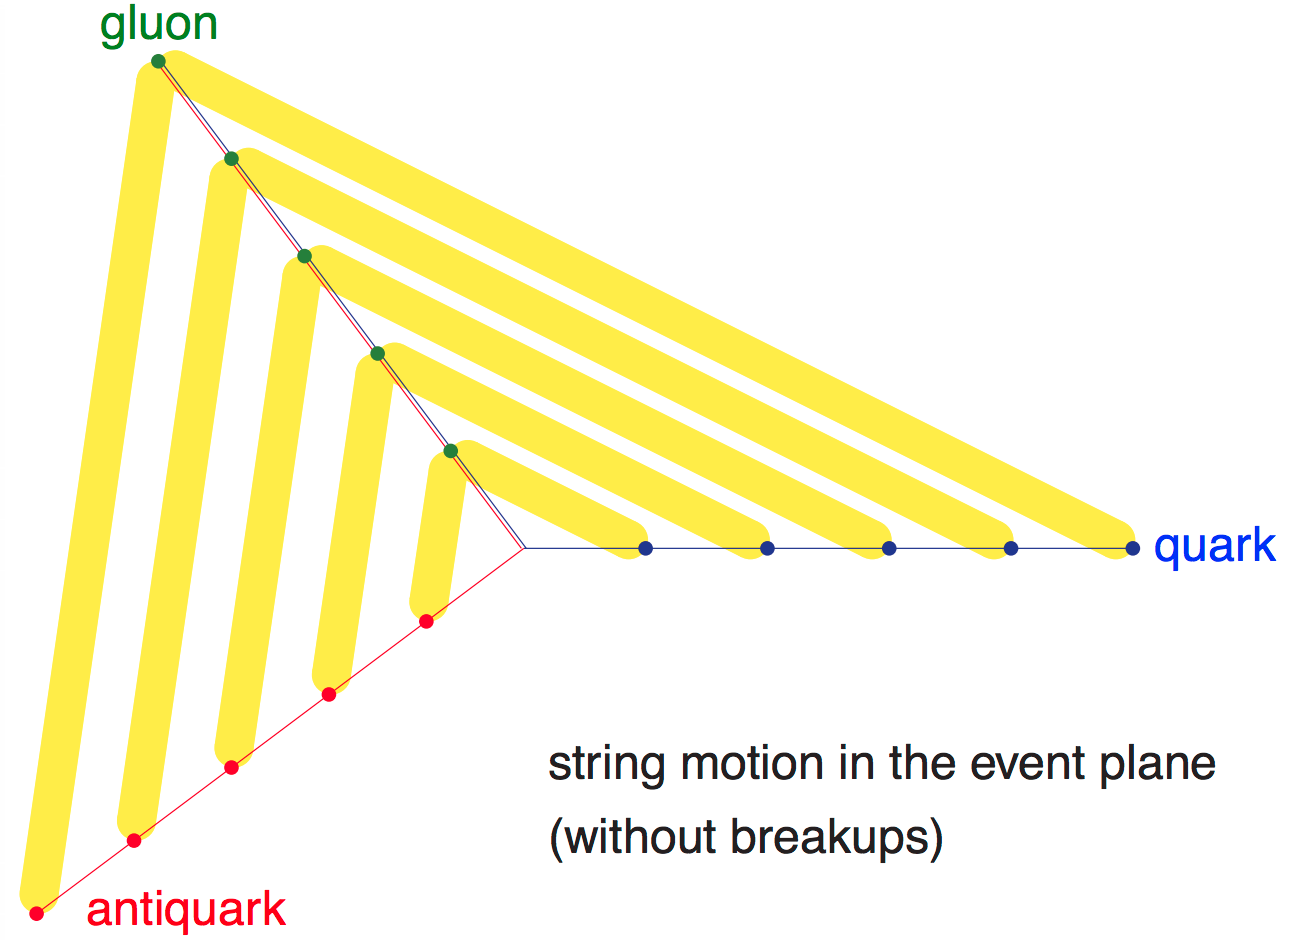
\includegraphics[width=0.43\textwidth]{Figures/Generator_Lund2}
	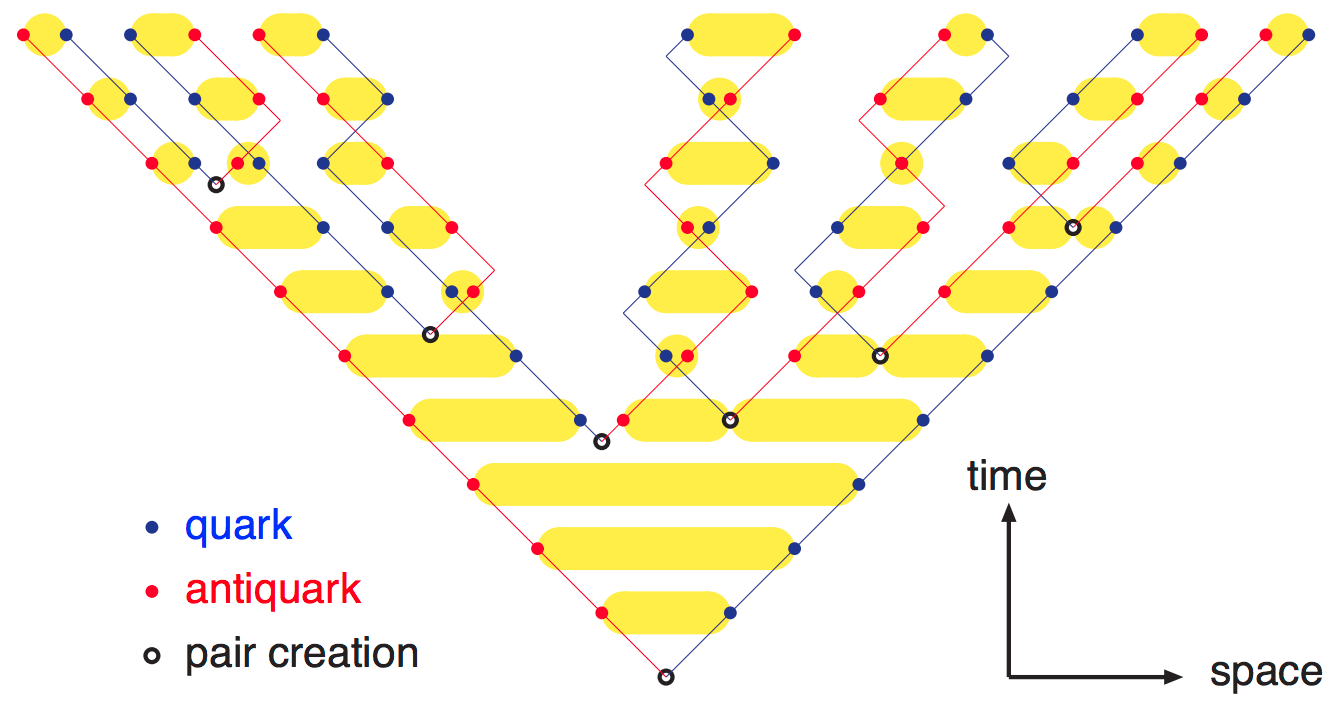
\includegraphics[width=0.56\textwidth]{Figures/Generator_Lund}
	\caption[The left panel shows the string between the quark-antiquark colour dipole stretched by a gluon and the right panel shows for each string how fragmentation occurs with time. Lorentz boosts in the hadrons are shown by oscillation frequency. ]{The left panel shows the string between the quark-antiquark colour dipole stretched by a gluon and the right panel shows for each string how fragmentation occurs with time. Lorentz boosts in the hadrons are shown by oscillation frequency. Figures taken from~\cite{Gen:Lund}.}
	\label{fig:Lund}
\end{figure}
As time evolves, if \qqbar{} pairs do not have enough potential in the colour field to pair-produce they end up bound to each other forming the colourless mesons of the final state.
It is also possible for the potential in the colour field to be great enough to produce diquark-diantiquark pair instead of \qqbar{} with the end result being the formation of baryons instead of mesons.
This approach is used in the \pythia{} parton shower simulation.
% pg10 https://indico.cern.ch/event/564031/contributions/2279204/attachments/1326142/1990851/16-FNAL-pp.pdf

The string dynamics currently assume that the colour-flow modelled in the evolution of the parton shower from the hard interaction is independent from the colour-flow of the other parton showers produced by the \MPI{}s.
Indeed, each individual \MPI{} is assumed to operate in independent colour spaces.
In reality, all the individual interactions are superimposed on each other, with soft gluons connecting all the final state partons from all sources, redistributing colour across the full parton shower.
In the Lund string model this can have the effect of reorganising the strings produced in the parton shower.
This is modelled in simulation by a process known as \textit{colour reconnection} (\CR{}), which reconfigures the colour strings after the parton shower, but before the fragmentation.
Three different models which can be implemented using \pythia{} are described here.
% MPIs happen between protons radius == transverse size of the qcd string == non independent simulation

\subsubsection{MPI-based model} % (fold)
\label{sub:mpi_based_model}

The \textit{MPI-based} \CR{} model~\cite{Gen:GluonMove} calculates the reconnection probability for all gluons from lower-\pt{} interactions to be inserted into the colour-flow dipoles of a higher-\pt{} interaction.
Once all reconnections between \MPI{}s have been identified, the configuration in which the total colour string length is minimised is selected.
The \pythia{} parton shower simulation uses the \MPI{}-based \CR{} scheme as default, where it is assumed that the lifetime of the top quark is long enough to shield the top decay products from the effects of \CR{}.
A second \MPI{}-based model exists where the top quark decays before the \CR{} is applied and as such the top decay products are able to reconnect.
This is known as \MPI{}-based \CR{} with \textit{early resonance decays} (erdON).
% Prob is higher for lower pt MPIs due to increased wavefunctions, which leads to higher spread and chance to interfere.
% Starting at ordered high-pt, look at colour reconnections to lower MPIs. Gluons are inserted between MPIs in such a way to minimize string length.

% The \MPI{}-based \CR{} model takes \MPI{}s, iterating in order of increasing hardness, and calculates a reconnection probability to \MPI{} with the next highest \pt{}.
% If no reconnection is found, consecutively harder \MPI{}s are tested.
% ERD: The \textit{gluon move/flip} model \cite{Gen:GluonMove} of the \CR{} starts from the default \MPI{}-based model. 
% The top quarks then decay and radiate, from which a second set of \CR{} occurs between radiated gluons from the top decay and those from the rest of the parton shower.
% subsubsection mpi_based_model (end)

\subsubsection{QCD-inspired model} % (fold)
\label{sub:qcd_inspired_model}

An alternative \CR{} model is the \textit{QCD-inspired} model~\cite{Gen:QCDBased}.
In this model, instead of the $\mathrm{SU(3)}$ colour indices ($r,g,b$) being applied to individual partons, a set of nine indices, which describe the possible colour states of 2-parton and 3-parton combinations, are used.
A corresponding set of anti-colour indices is used for anti-quarks and a gluon contains one of each index.
Reconnections are possible when two partons have a matching colour and anti-colour index.
The set of possible reconnections encompasses every possible reconnection from the default \MPI-based \CR{} model as well as reconnections possible between partons with accidentally matching colour indices.
As with the \MPI-based \CR{} model, a reconnection is performed if it minimises the total \QCD{} string length.
% subsubsection qcd_inspired_model (end)

\subsubsection{Gluon move/flip model} % (fold)
\label{sub:gluon_move_flip_model}

The \textit{gluon move/flip} model~\cite{Gen:GluonMove}, moves all final state gluons between colour strings so that the total string length is minimised. 
However, by moving only gluons, no quarks are able to reconnect and so a subsequent procedure is applied in which two colour segments are flipped between colour strings.
As with moving the gluons, the solution which minimises the total string length is used.
% a subset of final state gluons can be used given by a colour reconnection strength parameter.
% subsubsection gluon_move_flip_model (end)
% subsection string_fragmentation (end)
% section colour_reconnection (end)


\subsection{Cluster fragmentation model} % (fold)
\label{sub:cluster_fragmentation}

In the cluster model of fragmentation implemented in the \herwig{} parton shower simulation, all partons are showered until they reach an energy scale of $\sim4\GeV$, where hadronisation effects become non-negligible.
The final state gluons must have an energy at least twice that of the invariant mass of the lightest quark and are forced to split into a \qqbar{} pair.
The colour singlet states formed by the resulting colour connected partons are formed into clusters, as shown in Fig.~\ref{fig:Cluster}.
The cluster model assumes the principle of \textit{colour-preconfinement} which states that the distribution of the mass of the clusters is independent of the centre-of-mass energy and the hard scattering process involved.
Most clusters are distributed at low masses and can be regarded as excited hadron resonances and decayed into observed hadrons, however some clusters are too massive for this to be realistic and split in a process called \textit{cluster fission}.
If fission is required, a \qqbar{} pair of \uquark{}, \dquark{} or \squark{} flavour, is taken from the vacuum and the cluster split such that one of the original quarks is contained in each new cluster.
Fissions continue until all clusters are accepted by the mass parameters of the model.
The final process of the fragmentation involves extracting a \qqbar{} or \qqqbarqbar{} from vacuum in each cluster, forming a pair of hadrons, which in turn may decay into lighter hadrons.

\begin{figure}[htpb]
	\centering
	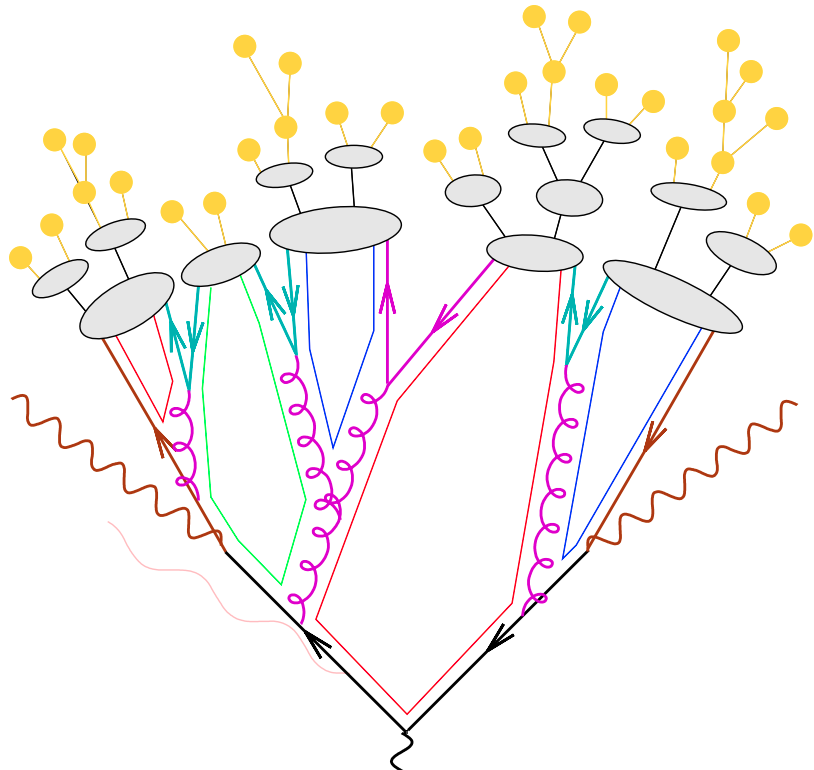
\includegraphics[width=0.6\textwidth]{Figures/Generator_Cluster}
	\caption[A sketch of the cluster model of fragmentation and hadronisation. Colour singlet clusters are generated from the final state quarks and gluons forced to split into a \quark{}\antiquark{} pair. These colour singlet clusters can be unnaturally massive and fission occurs until the clusters represent excited hadron resonances which then hadronise. ]{A sketch of the cluster model of fragmentation and hadronisation. Colour singlet clusters are generated from the final state quarks and gluons forced to split into a \quark{}\antiquark{} pair. These colour singlet clusters can be unnaturally massive and fission occurs until the clusters represent excited hadron resonances which then hadronise.  Figure adapted from \cite{Gen:Cluster}.}
	\label{fig:Cluster}
\end{figure}
% For cluster model, to conserve colour - intial partons must come from valence. gluon -> valence and emits anti quark. seaquark -> gluon -> valence. remnent qq collur triplet, valence: colour triplet
% gluon splitting to diquark pair not suported
% M^Clpow ≥ Clmax^Clpow + (m1 + m2)^Clpow. Clmax: max cluster mass. Clpow: mass exponent. m1,2 mass of cluster quark compentents
% the masses of the daughter clusters are required to be less than that of the parent cluster and greater than the sum of the masses of their constituent partons.
% flavour mixing in light hadrons.
% all probabilities depend on phase space. complicated and covered by model parameters

% subsection cluster_fragmentation (end)



% \begin{equation}
% 	\frac{dP}{d\pt} \propto \kappa (e^{\frac{\pi m_{\mathrm{T}}^2}{\kappa}})
% \end{equation}
% Dont know where this is from ^
% section fragmentation_and_colour_reconnection (end)





\section{Detector modelling} % (fold)
\label{sec:detector_modelling}

So far, only the modelling of the physics process itself has been discussed, before any interaction with the detector has been performed.
Indeed, it is very useful to compare measurements at this level, the \textit{particle level}, as it allows direct comparisons between theoretical models and experimental measurements which have had the detector response removed.
The removal of the detector response is discussed in Ch.~\ref{ch:unfolding}.
This means measurements performed to particle level with different detectors such as \CMS{} and ATLAS can be directly compared with each other and to theoretical predictions.

In order to provide the mapping between experiment and particle level, the detector response needs to be modelled accurately.
To do this a simulation toolkit called \textit{GEometry ANd Tracking} (\GEANT{})~\cite{Gen:GEANT} is used.
The \GEANT{} package builds the physical layout of the experiment, including all detectors, absorbers, electronics and structural components surrounding the central interaction point.
The magnetic field strength at all points in the detector is modelled.
The particles are tracked from the collision point outwards through the active and non-active material, modelling respective interactions and decays.
In the active material, the response of all individual components is modelled in a process known as \textit{digitisation}.
The digitisation takes into account any inefficiencies in the active material and returns an output consistent with that seen from measured data.
A full description of the \CMS{} detector is given in Ch.~\ref{ch:LHCCMS}.

% Not quite -phase space issues.
% section detector_modelling (end)

\section{Production of $\mathbf{\ttbar}$ and background models}
\label{sec:ttMC}

Table~\ref{tb:Gen} shows the complete set of simulations used for the differential cross section analysis performed.
There are four different \ttbar{} production models studied.
Two \ttbar{} samples are simulated with the \powheg{} (v2) matrix element generator~\cite{Gen:PowHVF}, where one sample is interfaced with \pythia{} (v8.212), using the \CUET{} tune~\cite{Gen:CUETP8M2T4}, and the second with the \herwig{} (v2.7.1) using the \herwigtune{} tune~\cite{Gen:EE5C}.
These are labelled \powhegpythia{} and \powhegherwig{} respectively.
Two additional simulated \ttbar samples are produced with the \mgamc{} (v2.2.2) generator.
One is used to generate events at \LO{} accuracy with up to three additional partons and the second to \NLO{} accuracy with up to two additional partons.
Both are interfaced with \pythia{} using the \CUETold{} tune~\cite{Gen:CUETP8M1} and are labelled \mgamcLO{} and \mgamcNLO{} respectively.
The \MLM{} jet-parton matching algorithm is used to match the matrix-element to the parton shower in the \LO{} simulation and the \FxFx{} algorithm in the \NLO{} simulation.
The \powhegpythia{} model is taken as the central model used in this thesis.

All \ttbar{} production samples are simulated with the top quark mass set to 172.5\GeV{}.
For \NLO{} samples the \nnpdf{} \PDF{} set~\cite{Gen:NNPDF} is used, while for \LO{} samples the \nnpdflo{} set is used.
The samples are normalised to a \NNLO{} \ttbar{} cross section of 832\pb{}, as seen in Sec.~\ref{sub:top_quark_production}.
It is important to compare multiple \ttbar{} generators in order to find the current most suitable description of top quark production and decay, and to identify any discrepancies in the models.

Table~\ref{tb:Gen} also shows the dominant background samples from single top quark production, vector boson production with associated jets and multi-jet \QCD{} production.
All the single top quark processes produced via the $t$-channel and in association with a \Wboson{}~boson are generated with \powheg{}~\cite{Gen:Pow_tchan,Gen:Pow_tWchan} interfaced with \pythia and are normalised to cross sections that are calculated to \NLO{} precision~\cite{Gen:ST_XSECPred_1,Gen:ST_XSECPred_2}.  
Samples of \Wboson{}{} and \Zboson{}~boson production in association with jets, with leptonic final states, are generated at \LO{} using \mgamc{}. 
Separate samples are generated with exactly one, two, three, and four additional jets to ensure a large set of background events.
These samples are normalized to their \NNLO{} cross sections~\cite{Gen:VJets_XSECPred}.
Multijet \QCD{} events are generated using \pythia{} for both the matrix-element calculations and parton shower/hadronisation.
Only multijet \QCD{} events with large electromagnetic activity or that contain a muon are generated in order to maximise the available sample size.

The simulated samples need to contain enough events to ensure they are not affected by statistical fluctuations when comparing to the data.
The luminosity, described in further detail in Sec.~\ref{sec:lumi}, produced for each simulation sample is shown in the final column of Tab.~\ref{tb:Gen} and should ideally be comparable to or larger than the luminosity of the data collected.
Looking ahead to Tab.~\ref{tb:Data2016}, the total collected data luminosity is 35.9\fbinv{} and so most of the signal and background samples do indeed contain enough events.
The multijet \QCD{} events are not particularly well modelled and can suffer from a lack of statistics and so a data-driven multijet \QCD{} estimate is employed, which is described in Sec.~\ref{sec:multijet_qcd}.
The multijet \QCD{} samples are still required in the creation of the estimate however.

Samples are also generated for variations of some of the generator parameters in \powhegpythia{}.
These are shown in Tab.~\ref{tb:GenSys} and are used as part of the estimation of the theoretical uncertainties due to the modelling.
Other theoretical uncertainties in the modelling are calculated as event weights and stored in the central \powhegpythia{} sample.
The CMS detector response for all simulated samples is modelled using \GEANT{}.

\begin{table}
	\centering
		\caption{The set of simulated samples used in this thesis. They include four different signal \ttbar{} production samples and samples for the background production. The backgrounds are single top quark production, vector boson production in association with jets and multijet \QCD{}. }
		\label{tb:Gen}
		\resizebox{\linewidth}{!}{%
		\begin{tabular}{llllccc}
			 	& \textbf{Matrix}	& \textbf{Parton} & \textbf{Tune}	& \textbf{Cross section} 	  			& \textbf{Events}  	& \textbf{Luminosity} 	\\
			 	& \textbf{element}	& \textbf{shower} &  				& \textbf{(\pb{})} 	&  	\textbf{(\ten{6})}	& \textbf{(\fbinv{})} 	\\
			\multicolumn{7}{l}{\textbf{Models of \ttbar{} production}} \\
			\hline
			\vspace*{0.02cm}
			\powhegpythia{} & \powheg{} & \pythia{} & \CUET{}		& 831.76 & 154.9 & 186.3 \\ 
			\powhegherwig{} & \powheg{} & \herwig{} & \herwigtune{}	& 831.76 & 59.2  & 77.1 \\ 
			\mgamcLO{} 		& \mgamc{}	& \pythia{} & \CUETold{}  	& 831.76 & 10.1  & 12.2 \\ 
			\mgamcNLO{} 	& \mgamc{}	& \pythia{} & \CUETold{}  	& 831.76 & 30.4  & 36.6 \\ 

			\vspace*{0.02cm} \\
			\multicolumn{7}{l}{\textbf{Models of single top background production}} \\
			\hline
			\vspace*{0.02cm}
			Single top $t$-channel 			& \powheg{} 			& \pythia{} &	\CUETold{}  & 136.02	  & 66.9  & 492.0 \\ 
			Single anti-top $t$-channel	 	& \powheg{} 			& \pythia{} &	\CUETold{}  & 80.95	  	  & 38.8  & 479.4 \\ 
			Single top $tW$-channel 		& \powheg{} (v1)		& \pythia{} &	\CUETold{}  & 35.6		  & 7.9   & 223.2 \\ 
			Single anti-top $tW$-channel 	& \powheg{} (v1)		& \pythia{} &	\CUETold{}  & 35.6		  & 7.9   & 222.8 \\ 
			Single top/anti-top $s$-channel & \mgamc{} 				& \pythia{} &	\CUETold{}  & 6.35		  & 0.6    & 98.1 \\ 

			\vspace*{0.02cm} \\
			\multicolumn{7}{l}{\textbf{Models of vector boson background production}} \\
			\hline 
			\vspace*{0.01cm}
			Drell-Yan + 1 jet 			& \mgamc{}			& \pythia{} &	\CUETold{}	 & 	1016		  &  62.6  & 61.6 \\ 
			Drell-Yan + 2 jets  		& \mgamc{}			& \pythia{} &	\CUETold{}	 & 	331.4		  &  20.0  & 60.3 \\ 
			Drell-Yan + 3 jets  		& \mgamc{}			& \pythia{} &	\CUETold{}	 & 	96.36		  &  5.9   & 60.8 \\ 
			Drell-Yan + 4 jets  		& \mgamc{}			& \pythia{} &	\CUETold{}	 & 	51.4		  &  4.2   & 81.7 \\ 
			\Wboson{} boson + 1 jet 	& \mgamc{}			& \pythia{} &	\CUETold{}	 & 	9493		  &  45.4  & 4.8 \\ 
			\Wboson{} boson + 2 jets 	& \mgamc{}			& \pythia{} &	\CUETold{}	 & 	3120		  &  60.2  & 19.3 \\ 
			\Wboson{} boson + 3 jets 	& \mgamc{}			& \pythia{} &	\CUETold{}	 & 	942.3		  &  59.1  & 62.7 \\ 
			\Wboson{} boson + 4 jets 	& \mgamc{}			& \pythia{} &	\CUETold{}	 & 	524.2		  &  30.0  & 57.2 \\ 

			\vspace*{0.02cm} \\
			\multicolumn{7}{l}{\textbf{Models of multijet \QCD{} background production}} \\
			\hline 
			\vspace*{0.02cm}
			Muon enriched \QCD (20-30) 			& \pythia{}			& \pythia{} &	\CUETold{}	 & 	558528000 * 0.0053		  &  30.6  & 0.01 \\ 
			Muon enriched \QCD (30-50) 			& \pythia{}			& \pythia{} &	\CUETold{}	 & 	139803000 * 0.01182		  &  30.0  & 0.02 \\ 
			Muon enriched \QCD (50-80) 			& \pythia{}			& \pythia{} &	\CUETold{}	 & 	19222500 * 0.02276		  &  19.8  & 0.04 \\ 
			Muon enriched \QCD (80-120) 		& \pythia{}			& \pythia{} &	\CUETold{}	 & 	2758420 * 0.03844		  &  23.6  & 0.2 \\ 
			Muon enriched \QCD (120-170) 		& \pythia{}			& \pythia{} &	\CUETold{}	 & 	469797 * 0.05362		  &  8.0  & 0.3 \\ 
			Muon enriched \QCD (170-300) 		& \pythia{}			& \pythia{} &	\CUETold{}	 & 	117989 * 0.07335		  &  17.4  & 2.0 \\ 
			Muon enriched \QCD (300-470) 		& \pythia{}			& \pythia{} &	\CUETold{}	 & 	7820.25 * 0.10196		  &  49.0  & 61.4 \\ 
			Muon enriched \QCD (470-600) 		& \pythia{}			& \pythia{} &	\CUETold{}	 & 	645.528 * 0.12242		  &  19.0  & 240.1 \\ 
			Muon enriched \QCD (600-800) 		& \pythia{}			& \pythia{} &	\CUETold{}	 & 	187.109 * 0.13412		  &  10.0  & 397.7 \\ 
			Muon enriched \QCD (800-1000) 		& \pythia{}			& \pythia{} &	\CUETold{}	 & 	32.3486 * 0.14552		  &  19.8  & 4199.3 \\ 
			Muon enriched \QCD (1000-Inf) 		& \pythia{}			& \pythia{} &	\CUETold{}	 & 	10.4305 * 0.15544		  &  13.4  & 8264.9 \\

			Electron enriched \QCD (20-30) 		& \pythia{}			& \pythia{} &	\CUETold{}	 & 557600000 * 0.0096		  & 9.2  & 0.002 \\ 
			Electron enriched \QCD (30-50) 		& \pythia{}			& \pythia{} &	\CUETold{}	 & 136000000 * 0.073		  & 6.8  & 0.0007 \\ 
			Electron enriched \QCD (50-80) 		& \pythia{}			& \pythia{} &	\CUETold{}	 & 19800000 * 0.146			  & 45.2  & 0.02 \\ 
			Electron enriched \QCD (80-120) 	& \pythia{}			& \pythia{} &	\CUETold{}	 & 2800000 * 0.125			  & 76.5  & 0.2 \\ 
			Electron enriched \QCD (120-170) 	& \pythia{}			& \pythia{} &	\CUETold{}	 & 477000 * 0.132			  & 77.8  & 1.2 \\ 
			Electron enriched \QCD (170-300) 	& \pythia{}			& \pythia{} &	\CUETold{}	 & 114000 * 0.165			  & 11.5  & 0.6 \\ 
			Electron enriched \QCD (300-Inf) 	& \pythia{}			& \pythia{} &	\CUETold{}	 & 9000 * 0.15			 	  & 7.4  & 54.6 \\ 
			
			bc to E \QCD (30-80) 				& \pythia{}			& \pythia{} &	\CUETold{}	 & 	159068000 * 0.00255 & 15.3   & 0.04 \\ 
			bc to E \QCD (80-170) 				& \pythia{}			& \pythia{} &	\CUETold{}	 & 	3221000 * 0.01183  	& 14.9   & 0.4 \\ 
			bc to E \QCD (170-250) 				& \pythia{}			& \pythia{} &	\CUETold{}	 & 	105771 * 0.02492  	& 9.7   & 3.9 \\ 
			bc to E \QCD (250-Inf) 				& \pythia{}			& \pythia{} &	\CUETold{}	 & 	21094.1 * 0.03375 	& 9.8   & 13.7 \\ 
		\end{tabular}%
	}
\end{table}

			% \powhegpythia{} & \powheg{} & \pythia{} & \CUET{}		& 831.76 & 154948894 & 186.3 \\ 
			% \powhegherwig{} & \powheg{} & \herwig{} & \herwigtune{}	& 831.76 & 59174465  & 77.1 \\ 
			% \mgamcLO{} 		& \mgamc{}	& \pythia{} & \CUETold{}  	& 831.76 & 10139950  & 12.2 \\ 
			% \mgamcNLO{} 	& \mgamc{}	& \pythia{} & \CUETold{}  	& 831.76 & 30414083  & 36.6 \\ 
			% Single top $t$-channel 			& \powheg{} 			& \pythia{} &	\CUETold{}  & 136.02	  & 66928232  & 492.0 \\ 
			% Single anti-top $t$-channel	 	& \powheg{} 			& \pythia{} &	\CUETold{}  & 80.95	  	  & 38811017  & 479.4 \\ 
			% Single top $tW$-channel 		& \powheg{} (v1)		& \pythia{} &	\CUETold{}  & 35.6		  & 7944854   & 223.2 \\ 
			% Single anti-top $tW$-channel 	& \powheg{} (v1)		& \pythia{} &	\CUETold{}  & 35.6		  & 7931370   & 222.8 \\ 
			% Single top/anti-top $s$-channel & \mgamc{} 				& \pythia{} &	\CUETold{}  & 6.35		  & 622990    & 98.1 \\ 
			% Drell-Yan + 1 jet 			& \mgamc{}			& \pythia{} &	\CUETold{}	 & 	1016		  &  62627174  & 61.6 \\ 
			% Drell-Yan + 2 jets  		& \mgamc{}			& \pythia{} &	\CUETold{}	 & 	331.4		  &  19970551  & 60.3 \\ 
			% Drell-Yan + 3 jets  		& \mgamc{}			& \pythia{} &	\CUETold{}	 & 	96.36		  &  5856110   & 60.8 \\ 
			% Drell-Yan + 4 jets  		& \mgamc{}			& \pythia{} &	\CUETold{}	 & 	51.4		  &  4197868   & 81.7 \\ 
			% \Wboson{} boson + 1 jet 	& \mgamc{}			& \pythia{} &	\CUETold{}	 & 	9493		  &  45367044  & 4.8 \\ 
			% \Wboson{} boson + 2 jets 	& \mgamc{}			& \pythia{} &	\CUETold{}	 & 	3120		  &  60197766  & 19.3 \\ 
			% \Wboson{} boson + 3 jets 	& \mgamc{}			& \pythia{} &	\CUETold{}	 & 	942.3		  &  59067548  & 62.7 \\ 
			% \Wboson{} boson + 4 jets 	& \mgamc{}			& \pythia{} &	\CUETold{}	 & 	524.2		  &  29995313  & 57.2 \\ 
			% Muon enriched \QCD (20-30) 			& \pythia{}			& \pythia{} &	\CUETold{}	 & 	558528000 * 0.0053		  &  30613738  & 0.01 \\ 
			% Muon enriched \QCD (30-50) 			& \pythia{}			& \pythia{} &	\CUETold{}	 & 	139803000 * 0.01182		  &  29954815  & 0.02 \\ 
			% Muon enriched \QCD (50-80) 			& \pythia{}			& \pythia{} &	\CUETold{}	 & 	19222500 * 0.02276		  &  19806915  & 0.04 \\ 
			% Muon enriched \QCD (80-120) 		& \pythia{}			& \pythia{} &	\CUETold{}	 & 	2758420 * 0.03844		  &  23584215  & 0.2 \\ 
			% Muon enriched \QCD (120-170) 		& \pythia{}			& \pythia{} &	\CUETold{}	 & 	469797 * 0.05362		  &  8042721  & 0.3 \\ 
			% Muon enriched \QCD (170-300) 		& \pythia{}			& \pythia{} &	\CUETold{}	 & 	117989 * 0.07335		  &  17350231  & 2.0 \\ 
			% Muon enriched \QCD (300-470) 		& \pythia{}			& \pythia{} &	\CUETold{}	 & 	7820.25 * 0.10196		  &  48995686  & 61.4 \\ 
			% Muon enriched \QCD (470-600) 		& \pythia{}			& \pythia{} &	\CUETold{}	 & 	645.528 * 0.12242		  &  18976018  & 240.1 \\ 
			% Muon enriched \QCD (600-800) 		& \pythia{}			& \pythia{} &	\CUETold{}	 & 	187.109 * 0.13412		  &  9981311  & 397.7 \\ 
			% Muon enriched \QCD (800-1000) 		& \pythia{}			& \pythia{} &	\CUETold{}	 & 	32.3486 * 0.14552		  &  19767439  & 4199.3 \\ 
			% Muon enriched \QCD (1000-Inf) 		& \pythia{}			& \pythia{} &	\CUETold{}	 & 	10.4305 * 0.15544		  &  13400031  & 8264.9 \\
			% Electron enriched \QCD (20-30) 		& \pythia{}			& \pythia{} &	\CUETold{}	 & 557600000 * 0.0096		  & 9218954  & 0.002 \\ 
			% Electron enriched \QCD (30-50) 		& \pythia{}			& \pythia{} &	\CUETold{}	 & 136000000 * 0.073		  & 6768384  & 0.0007 \\ 
			% Electron enriched \QCD (50-80) 		& \pythia{}			& \pythia{} &	\CUETold{}	 & 19800000 * 0.146			  & 45156163  & 0.02 \\ 
			% Electron enriched \QCD (80-120) 	& \pythia{}			& \pythia{} &	\CUETold{}	 & 2800000 * 0.125			  & 76489397  & 0.2 \\ 
			% Electron enriched \QCD (120-170) 	& \pythia{}			& \pythia{} &	\CUETold{}	 & 477000 * 0.132			  & 77771316  & 1.2 \\ 
			% Electron enriched \QCD (170-300) 	& \pythia{}			& \pythia{} &	\CUETold{}	 & 114000 * 0.165			  & 11540163  & 0.6 \\ 
			% Electron enriched \QCD (300-Inf) 	& \pythia{}			& \pythia{} &	\CUETold{}	 & 9000 * 0.15			 	  & 7373633  & 54.6 \\ 
			% bc to E \QCD (30-80) 				& \pythia{}			& \pythia{} &	\CUETold{}	 & 	159068000 * 0.00255 & 15328096   & 0.04 \\ 
			% bc to E \QCD (80-170) 				& \pythia{}			& \pythia{} &	\CUETold{}	 & 	3221000 * 0.01183  	& 14976689   & 0.4 \\ 
			% bc to E \QCD (170-250) 				& \pythia{}			& \pythia{} &	\CUETold{}	 & 	105771 * 0.02492  	& 9720760   & 3.9 \\ 
			% bc to E \QCD (250-Inf) 				& \pythia{}			& \pythia{} &	\CUETold{}	 & 	21094.1 * 0.03375 	& 9773617   & 13.7 \\ 




\begin{table}
	\centering
		\caption{The set of samples associated with the uncertainties in the \powhegpythia{} modelling. Other uncertainties are modelled by the use of event weights in the central \powhegpythia{} simulation.}
		\label{tb:GenSys}
		% \resizebox{\linewidth}{!}{%
		\begin{tabular}{lcc}
			\textbf{Variation}	& \textbf{Events}	& \textbf{Luminosity} \\
								& \textbf{(\ten{6})}	& \textbf{(\fbinv{})} \\
			\hline
			\ISR{} down						& 59.0 & 70.9 \\
			\ISR{} up						& 59.0 & 71.0 \\ 
			\FSR{} down						& 59.3 & 71.3 \\
			\FSR{} up						& 59.2 & 71.2 \\ 
			Underlying event down			& 58.3 & 70.1 \\ 
			Underlying event up				& 59.0 & 70.9 \\ 
			Matching scale (\hdamp{}) down	& 58.2 & 69.9 \\
			Matching scale (\hdamp{}) up	& 58.9 & 70.8 \\ 
			\CR{} \MPI{}-based erdON 		& 59.9 & 72.0 \\ 
			\CR{} \QCD{}-inspired 			& 59.6 & 71.7 \\ 
			\CR{} Gluon move 				& 59.0 & 71.0 \\ 
			Top quark mass (169.5\GeV{})	& 59.5 & 70.4 \\
			Top quark mass (175.5\GeV{})	& 59.4 & 71.4 \\
		\end{tabular}%
	% }
\end{table}

			% \hline
			% \ISR{} down						& 58999580 & 70.9 \\
			% \ISR{} up						& 59033604 & 71.0 \\ 
			% \FSR{} down						& 59306906 & 71.3 \\
			% \FSR{} up						& 59230899 & 71.2 \\ 
			% Underlying event down			& 58338240 & 70.1 \\ 
			% Underlying event up				& 58953660 & 70.9 \\ 
			% Matching scale (\hdamp{}) down	& 58163976 & 69.9 \\
			% Matching scale (\hdamp{}) up	& 58858606 & 70.8 \\ 
			% \CR{} \MPI{}-based erdON 		& 59882210 & 72.0 \\ 
			% \CR{} \QCD{}-inspired 			& 59620206 & 71.7 \\ 
			% \CR{} Gluon move 				& 59037234 & 71.0 \\ 
			% Top quark mass (169.5\GeV{})	& 58542590 & 70.4 \\
			% Top quark mass (175.5\GeV{})	& 59384660 & 71.4 \\

% In this sample, the diagram removal scheme~\cite{DiagramRemoval} is used to avoid double counting of Feynman diagrams in the production of single top quarks in association with a \Wboson{}~boson at \NLO and top quark pair production.

% A set of additional samples reflecting some of the uncertainties in the central \powhegpythia{} model are also used.
% Other uncertainties in the model such as TODO are supplied as weights in the \powhegpythia{} model.



% \begin{itemize}
% 	\item TODO: ALL OF THE REFS
% 	\item TODO: LUND MESON-BARYON RATIO
% 	\item TODO: MATRIX ELEMENT DEF HERE OR PREV CHAP
% 	\item TODO: LOOPS LEAD TO POSITIVE WEIGHTS? MG5 CAN HAVE -VE
% 	\item TODO: IS \ISR{} BREHMSSTRAHLUNG?
% 	\item TODO: pp vs gg cross section
% 	\item TODO: MATCHING BETWEN POWHEG AND PYTHIA/HERWIG
% \end{itemize}
